\section{Anatomy and structure of websites and web pages}\label{sec:structure_of_the_web}

\subsection{Structure of a website}\label{subsec:structure-of-a-website}

The structure of a web page generally follows one of four structural models\cite{Reyes_2025}.
\begin{enumerate}

    \item \textbf{Hierarchical (tree structure)}: This is the most common model, mirroring human cognitive processes and the way we organize information.
    It consists of a root node (the homepage) with branches leading to category pages, which further branch out to product pages and other content.
    This structure is intuitive for users and allows for easy navigation.

    \item \textbf{Sequential (linear structure)}: In this model, pages are arranged in a linear sequence, often used for storytelling or step-by-step guides.
    Users navigate through the content in a predetermined order, which can be effective for certain types of content but may limit user freedom.
    This style is common in e-commerce checkout processes, where users are guided through a series of steps to complete a purchase.

    \item \textbf{Matrix (grid structure)}: This model allows for multiple pathways between pages, with links connecting various nodes in a non-linear fashion.
    It is often used in content-rich websites, such as news sites or social media platforms, where users can navigate through different topics and categories without a strict hierarchy.

    \item \textbf{Database (dynamic structure)}: In this model, content is generated dynamically from a database based on user queries or interactions.
    It is common in e-commerce sites, where product pages are generated based on user searches or filters, and in social media platforms, where user-generated content is displayed based on relevance or popularity.
\end{enumerate}

\subsection{Anatomy of a web page}\label{subsec:anatomy-of-a-web-page}

A web page is collection of elements that are common components of the overall website (site-level components), and elements that are specific to the individual page (page-level components)\cite{WixPartsOfWebsite}.

\subsubsection{Site-level components}\label{subsubsec:site-level-components}
Site-level components are elements that are typically present across multiple pages of a website, providing consistency and aiding in navigation.
These include:
\begin{itemize}
    \item \textbf{Header}: The header is located at the top of the page and often contains the website's logo, navigation menu, search bar, and sometimes contact information or social media links.
    It serves as a consistent element across the site, allowing users to easily navigate to different sections of the website.
    \item \textbf{Footer}: The footer is located at the bottom of the page and often contains additional navigation links, contact information, copyright notices, and sometimes social media links.
    Like the header, it provides consistency across the site and can help users find important information or navigate to other sections.
\end{itemize}

\subsubsection{Page-level components}\label{subsubsec:page-level-components}
Page-level components are elements that are specific to the individual page and can vary widely depending on the type of page and its purpose.
These include:
\begin{itemize}
    \item \textbf{Main content area}: This is the central part of the page where the primary content is displayed.
    It can include text, images, videos, and other media, and is the main focus of the page.
    \item \textbf{Sidebar}: A sidebar is an additional column that can be located on either side of the main content area.
    It often contains supplementary information, such as related articles, advertisements, or additional navigation links.
    \item \textbf{Hero section}: A hero section is a prominent area at the top of the page, often featuring a large image or video, along with a headline and call-to-action button.
    It is designed to capture the user's attention and convey the main message or purpose of the page.
\end{itemize}

\subsection{HTML tags and the document object model (DOM)}\label{subsec:html_tags_and_dom}
HTML (HyperText Markup Language) is the standard language used to create and structure web pages.
It uses a system of tags to define the structure and content of a web page, allowing browsers to render the page correctly.
Semantic HTML involves the use of HTML tags such as \texttt{<header>}, \texttt{<nav>}, \texttt{<main>}, \texttt{<article>}, and \texttt{<footer>} to provide meaning to the content and structure of the page, which can improve accessibility and SEO (Search Engine Optimization).

The Document Object Model (DOM) is a programming interface for HTML and XML documents.
It represents the structure of a web page as a tree of nodes, where each node corresponds to an element in the HTML document.
The DOM allows developers to manipulate the content and structure of a web page dynamically using JavaScript, enabling interactive features and dynamic content updates without requiring a page reload\cite{ricca2000web}.

\begin{figure}[h]
    \centering
    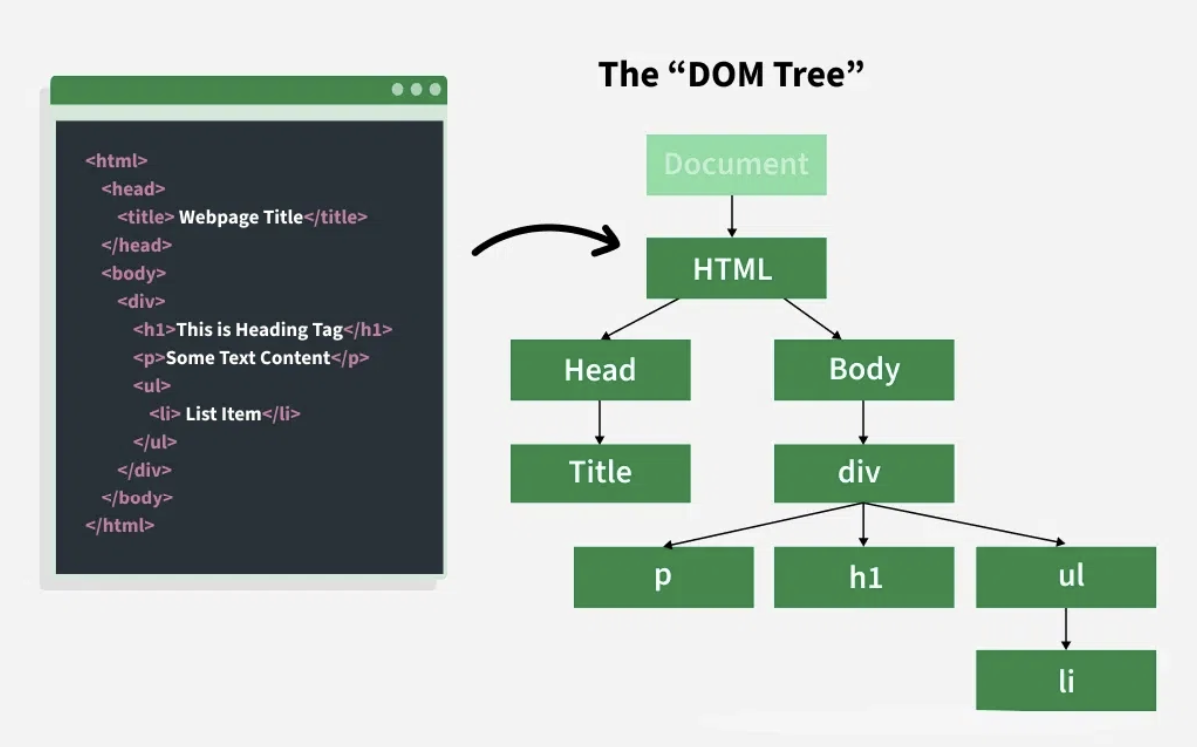
\includegraphics[width=0.8\textwidth]{images/html-and-dom}~\caption{HTML and the corresponding DOM tree\cite{GeeksforGeeksJavaScriptHTMLDOM}}
    \label{fig:html_and_dom}
\end{figure}

\subsection{Information hierarchy in e-commerce websites}\label{subsec:information_hierarchy_in_ecommerce_websites}
E-commerce sites are usually structured around a conversion funnel designed to move visitors from awareness to purchase\cite{YotpoEcommerceFunnel}.
\begin{itemize}
    \item \textbf{Homepage}: The homepage serves as the entry point to the website and provides an overview of the site's offerings, often featuring promotions, popular products, and links to key categories.
    It is designed to capture the user's attention and encourage them to explore further.

    \item \textbf{Product Listing Page (PLP)}: The PLP displays a list of products within a specific category or based on a search query.
    It typically includes filters and sorting options to help users find the products they are interested in.
    The PLP is designed to facilitate product discovery and encourage users to click through to individual product pages.

    \item \textbf{Product Detail Page (PDP)}: The PDP provides detailed information about a specific product, including images, descriptions, specifications, pricing, and customer reviews.
    It is designed to provide all the information a user needs to make a purchasing decision and often includes a call-to-action button to add the product to the cart or proceed to checkout.
\end{itemize}

\subsection{The semantic web and structured data}\label{subsec:semantic_web_and_structured_data}
The semantic web is an extension of the current web that aims to make data on the web more machine-readable and understandable by providing a standardized way to represent and link data using technologies such as RDF (Resource Description Framework) and OWL (Web Ontology Language).
Structured data is a way of annotating web content with specific tags and formats that provide additional context and meaning to the content, making it easier for search engines and other applications to understand and process the information on the web page.
One common format for structured data is JSON-LD (JavaScript Object Notation for Linked Data), which allows webmasters to embed structured data in a web page using a JSON format that is easy for both humans and machines to read and understand\cite{lanthaler2012using}.

In e-commerce websites, structured data can be used to provide detailed information about products, such as price, availability, reviews, and other attributes, which can enhance the visibility of the products in search engine results and improve the user experience by providing rich snippets in search results.

\begin{figure}[h]
    \centering
    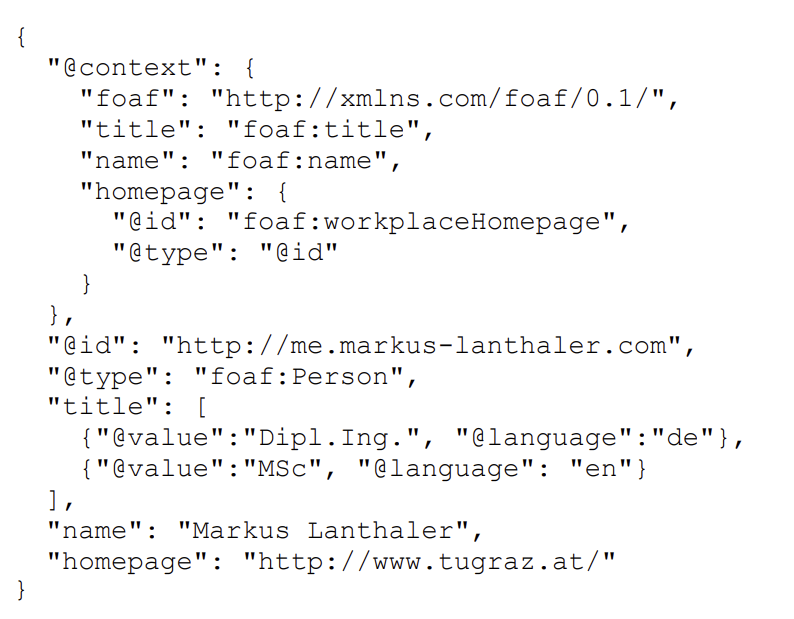
\includegraphics[width=0.8\textwidth]{images/json-ld-example}~\caption{Example of a JSON-LD document\cite{lanthaler2012using}}
    \label{fig:json_ld_example}
\end{figure}


% information hierarchy (homepage, category page, product page)
% anatomy of a website
% anatomy of a web page
% HTML tags and significance
% DOM structure
% static vs dynamic content
% the semantic web
% json-ld
